\documentclass[11pt,a4paper,]{article}
\usepackage{lmodern}

\usepackage{amssymb,amsmath}
\usepackage{ifxetex,ifluatex}
\usepackage{fixltx2e} % provides \textsubscript
\ifnum 0\ifxetex 1\fi\ifluatex 1\fi=0 % if pdftex
  \usepackage[T1]{fontenc}
  \usepackage[utf8]{inputenc}
\else % if luatex or xelatex
  \usepackage{unicode-math}
  \defaultfontfeatures{Ligatures=TeX,Scale=MatchLowercase}
\fi
% use upquote if available, for straight quotes in verbatim environments
\IfFileExists{upquote.sty}{\usepackage{upquote}}{}
% use microtype if available
\IfFileExists{microtype.sty}{%
\usepackage[]{microtype}
\UseMicrotypeSet[protrusion]{basicmath} % disable protrusion for tt fonts
}{}
\PassOptionsToPackage{hyphens}{url} % url is loaded by hyperref
\usepackage[unicode=true]{hyperref}
\hypersetup{
            pdftitle={Using Remote Sensing Data to Understand Fire Ignition During the 2019-2020 Australia Bushfire Season},
            pdfborder={0 0 0},
            breaklinks=true}
\urlstyle{same}  % don't use monospace font for urls
\usepackage{geometry}
\geometry{a4paper, centering, text={16cm,24cm}}
\usepackage[style=apa,]{biblatex}
\addbibresource{references.bib}
\usepackage{longtable,booktabs}
% Fix footnotes in tables (requires footnote package)
\IfFileExists{footnote.sty}{\usepackage{footnote}\makesavenoteenv{long table}}{}
\usepackage{graphicx,grffile}
\makeatletter
\def\maxwidth{\ifdim\Gin@nat@width>\linewidth\linewidth\else\Gin@nat@width\fi}
\def\maxheight{\ifdim\Gin@nat@height>\textheight\textheight\else\Gin@nat@height\fi}
\makeatother
% Scale images if necessary, so that they will not overflow the page
% margins by default, and it is still possible to overwrite the defaults
% using explicit options in \includegraphics[width, height, ...]{}
\setkeys{Gin}{width=\maxwidth,height=\maxheight,keepaspectratio}
\IfFileExists{parskip.sty}{%
\usepackage{parskip}
}{% else
\setlength{\parindent}{0pt}
\setlength{\parskip}{6pt plus 2pt minus 1pt}
}
\setlength{\emergencystretch}{3em}  % prevent overfull lines
\providecommand{\tightlist}{%
  \setlength{\itemsep}{0pt}\setlength{\parskip}{0pt}}
\setcounter{secnumdepth}{5}

% set default figure placement to htbp
\makeatletter
\def\fps@figure{htbp}
\makeatother


\title{Using Remote Sensing Data to Understand Fire Ignition During the 2019-2020 Australia Bushfire Season}

%% MONASH STUFF

%% CAPTIONS
\RequirePackage{caption}
\DeclareCaptionStyle{italic}[justification=centering]
 {labelfont={bf},textfont={it},labelsep=colon}
\captionsetup[figure]{style=italic,format=hang,singlelinecheck=true}
\captionsetup[table]{style=italic,format=hang,singlelinecheck=true}


%% FONT
\RequirePackage{bera}
\RequirePackage[charter,expert,sfscaled]{mathdesign}
\RequirePackage{fontawesome}

%% HEADERS AND FOOTERS
\RequirePackage{fancyhdr}
\pagestyle{fancy}
\rfoot{\Large\sffamily\raisebox{-0.1cm}{\textbf{\thepage}}}
\makeatletter
\lhead{\textsf{\expandafter{\@title}}}
\makeatother
\rhead{}
\cfoot{}
\setlength{\headheight}{15pt}
\renewcommand{\headrulewidth}{0.4pt}
\renewcommand{\footrulewidth}{0.4pt}
\fancypagestyle{plain}{%
\fancyhf{} % clear all header and footer fields
\fancyfoot[C]{\sffamily\thepage} % except the center
\renewcommand{\headrulewidth}{0pt}
\renewcommand{\footrulewidth}{0pt}}

%% MATHS
\RequirePackage{bm,amsmath}
\allowdisplaybreaks

%% GRAPHICS
\RequirePackage{graphicx}
\setcounter{topnumber}{2}
\setcounter{bottomnumber}{2}
\setcounter{totalnumber}{4}
\renewcommand{\topfraction}{0.85}
\renewcommand{\bottomfraction}{0.85}
\renewcommand{\textfraction}{0.15}
\renewcommand{\floatpagefraction}{0.8}


%\RequirePackage[section]{placeins}

%% SECTION TITLES


%% SECTION TITLES
\RequirePackage[compact,sf,bf]{titlesec}
\titleformat*{\section}{\Large\sf\bfseries\color[rgb]{0.7,0,0}}
\titleformat*{\subsection}{\large\sf\bfseries\color[rgb]{0.7,0,0}}
\titleformat*{\subsubsection}{\sf\bfseries\color[rgb]{0.7,0,0}}
\titlespacing{\section}{0pt}{2ex}{.5ex}
\titlespacing{\subsection}{0pt}{1.5ex}{0ex}
\titlespacing{\subsubsection}{0pt}{.5ex}{0ex}


%% TITLE PAGE
\def\Date{\number\day}
\def\Month{\ifcase\month\or
 January\or February\or March\or April\or May\or June\or
 July\or August\or September\or October\or November\or December\fi}
\def\Year{\number\year}

%% LINE AND PAGE BREAKING
\sloppy
\clubpenalty = 10000
\widowpenalty = 10000
\brokenpenalty = 10000
\RequirePackage{microtype}

%% PARAGRAPH BREAKS
\setlength{\parskip}{1.4ex}
\setlength{\parindent}{0em}

%% HYPERLINKS
\RequirePackage{xcolor} % Needed for links
\definecolor{darkblue}{rgb}{0,0,.6}
\RequirePackage{url}

\makeatletter
\@ifpackageloaded{hyperref}{}{\RequirePackage{hyperref}}
\makeatother
\hypersetup{
     citecolor=0 0 0,
     breaklinks=true,
     bookmarksopen=true,
     bookmarksnumbered=true,
     linkcolor=darkblue,
     urlcolor=blue,
     citecolor=darkblue,
     colorlinks=true}

\usepackage[showonlyrefs]{mathtools}
\usepackage[no-weekday]{eukdate}

%% BIBLIOGRAPHY

\makeatletter
\@ifpackageloaded{biblatex}{}{\usepackage[style=authoryear-comp, backend=biber, natbib=true]{biblatex}}
\makeatother
\ExecuteBibliographyOptions{bibencoding=utf8,minnames=1,maxnames=3, maxbibnames=99,dashed=false,terseinits=true,giveninits=true,uniquename=false,uniquelist=false,doi=false, isbn=false,url=true,sortcites=false}

\DeclareFieldFormat{url}{\texttt{\url{#1}}}
\DeclareFieldFormat[article]{pages}{#1}
\DeclareFieldFormat[inproceedings]{pages}{\lowercase{pp.}#1}
\DeclareFieldFormat[incollection]{pages}{\lowercase{pp.}#1}
\DeclareFieldFormat[article]{volume}{\mkbibbold{#1}}
\DeclareFieldFormat[article]{number}{\mkbibparens{#1}}
\DeclareFieldFormat[article]{title}{\MakeCapital{#1}}
\DeclareFieldFormat[article]{url}{}
%\DeclareFieldFormat[book]{url}{}
%\DeclareFieldFormat[inbook]{url}{}
%\DeclareFieldFormat[incollection]{url}{}
%\DeclareFieldFormat[inproceedings]{url}{}
\DeclareFieldFormat[inproceedings]{title}{#1}
\DeclareFieldFormat{shorthandwidth}{#1}
%\DeclareFieldFormat{extrayear}{}
% No dot before number of articles
\usepackage{xpatch}
\xpatchbibmacro{volume+number+eid}{\setunit*{\adddot}}{}{}{}
% Remove In: for an article.
\renewbibmacro{in:}{%
  \ifentrytype{article}{}{%
  \printtext{\bibstring{in}\intitlepunct}}}

\AtEveryBibitem{\clearfield{month}}
\AtEveryCitekey{\clearfield{month}}

\makeatletter
\DeclareDelimFormat[cbx@textcite]{nameyeardelim}{\addspace}
\makeatother

\author{\sf\Large\textbf{ Weihao Li}\\ {\sf\large EBS Honours student\\[0.5cm]}}

\date{\sf\Date~\Month~\Year}
\makeatletter
\lfoot{\sf Li: \@date}
\makeatother


%%%% PAGE STYLE FOR FRONT PAGE OF REPORTS

\makeatletter
\def\organization#1{\gdef\@organization{#1}}
\makeatother
  \organization{for Honours, supervised by Prof.~Di Cook}

  \def\name{Department of\newline Econometrics \&\newline Business Statistics}

\def\logo{
\includegraphics[width=6cm]{MBSportrait}}
\def\extraspace{\vspace*{1.6cm}}

%%%% FRONT PAGE OF REPORTS

\def\reporttype{Research Plan}

\long\def\front#1#2#3{
\newpage
\begin{singlespacing}
\thispagestyle{empty}
\vspace*{-1.4cm}
\hspace*{-1.4cm}
\hbox to 16cm{
  \hbox to 6.5cm{\vbox to 14cm{\vbox to 25cm{
    \logo
    \vfill
    \parbox{6.3cm}{\raggedright
      \sf\color[rgb]{0.00,0.00,0.70}
      {\large\textbf{\name}}\par
     }
  }\vss}\hss}
  \hspace*{0.2cm}
  \hbox to 1cm{\vbox to 14cm{\rule{1pt}{26.8cm}\vss}\hss\hfill}
  \hbox to 10cm{\vbox to 14cm{\vbox to 25cm{
      \vspace*{3cm}\sf\raggedright
      \parbox{11cm}{\sf\raggedright\baselineskip=1.2cm
         \fontsize{24.88}{30}\color[rgb]{0.70,0.00,0.00}\sf\textbf{#1}}
      \par
      \vfill
      \large
      \vbox{\parskip=0.8cm #2}\par
      \vspace*{2cm}\par
      {\large\textbf{\reporttype}}\\[0.3cm]
      \hbox{#3}%\\[2cm]\
      \vspace*{1cm}
      {\large\sf\textbf{\Date~\Month~\Year}}
   }\vss}
  }}
\end{singlespacing}
\newpage
}

\makeatletter
\def\titlepage{\front{\expandafter{\@title}}{\@author}{\@organization}}
\makeatother

\usepackage{setspace}
\setstretch{1.5}

%% Any special functions or other packages can be loaded here.
\usepackage{flafter}
\usepackage{booktabs}
\usepackage{longtable}
\usepackage{array}
\usepackage{multirow}
\usepackage{wrapfig}
\usepackage{float}
\usepackage{colortbl}
\usepackage{pdflscape}
\usepackage{tabu}
\usepackage{threeparttable}
\usepackage{threeparttablex}
\usepackage[normalem]{ulem}
\usepackage{makecell}
\usepackage{xcolor}


\begin{document}
\titlepage

\hypertarget{introduction}{%
\section{Introduction}\label{introduction}}

In Australia, bushfires have historically caused massive loss of property and life. Since the 1967 Hobart bushfires, the insurance claims for building losses was greater than \$A10 million \autocite{mcaneney2009100}.
The Australian bushfire season in 2019-2020, compared with other major bushfires in history, had a more devastating impact on the environment and properties. According to the report of \textcite{LisaRichardsNigelBrew2020} published by Parliament of Australia, 3094 houses have been destroyed and over 17M hectares of land burned in the last bushfire season. These two figures are the highest in history. Fortunately, only 33 people including firefighters died compared to 173 in the Black Saturday fires and 47 in Ash Wednesday fires \autocite{LisaRichardsNigelBrew2020}.
Understanding the cause of the 2019-2020 Australian bushfires is a crucial step to provide information for future policy and fire risk management.

The research is also motivated by the lack of knowledge about the cause of bushfire in Australia. \textcite{beale2011preventing} state in their research that the cause is only known for 58.9\% of fires. Historically, about 50\% are due to deliberate and suspicious ignitions, 35\% by accidents and 6\% natural, such as lightning. Providing a probable cause for bushfires may help investigators in practice.

\hypertarget{research-aims-and-questions}{%
\section{Research aims and questions}\label{research-aims-and-questions}}

This research will explore the potential methods of fire ignition during 2019-2020 Australia bushfires season based on the new availability of satellite data, and provide a model to predict the fire risk for locations around the country. Hotspots data from the JAXA's Himawari-8 satellite, will be combined with weather data from the Australian Bureau of Meteorology, and other data on roads, recreation sites, vegetation, to study locations of fire ignition and predict bushfire risk. Satellite data provides the opportunity to more objectively study ignition locations, particularly in less accessible regions.

The overall research aim is to provide probabilistic estimates of the cause of fire ignition for the 2019-2020 bushfires. Several smaller research questions that will be addressed are:

\begin{enumerate}
\def\labelenumi{\arabic{enumi}.}
\tightlist
\item
  Using satellite hotspots data can we detect ignition time and location?
\item
  Can data from other sources including vegetation, weather, proximity to road and recreation site help to inform ignition type?
\item
  How do the characteristics of 2019-2020 bushfires compare to historical bushfires?
\item
  Can we make a useful model for the fire risk across Australia? What predictors including fire indexes, proximity to road and recreation site, weather and vegetation are useful for modelling fire risk?
\end{enumerate}

\hypertarget{review-of-literature}{%
\section{Review of literature}\label{review-of-literature}}

Existing research on bushfire modelling can be divided into two main categories: simulation and analytical modelling.

In simulation modelling, \textcite{keane2004classification} develop landscape fire succession models (LFSMs) to simulate fire behaviour spatially, including fire ignition and fire spread, and accounting for fire and vegetation dynamics. \textcite{bradstock2012wildfires} used a model called FIRESCAPE which involved simulating fire behaviours with fuel and weather conditions. Simulation methods are cost-effective and time-effective ways to model bushfires, but ignition cause is not considered \autocite{clarke2019developing}. These methods seldomly address the ignition types that we are interested in.

Analytical modelling is another common way to build bushfires models. The general framework for analysing bushfires ignitions is a generalised additive model (GAM). \textcite{bates2018exploratory} used it with a Gaussian distribution for predicting the number of lightning ignitions. Some studies implemented GAM with a multinomial distribution to predict ignition probability \autocite{read2018lightning,zhang2017wildfire}. Mixed-effect models have also been considered to incorporate spatial dependence and weather factors \autocite{duff2018dryness}. Simpler models have also been used, including multiple linear regression, negative binomial regression and generalised logistic regression \autocite{cheney2012predicting,plucinski2014predicting,collins2015spatial}. Particularly, instead of using a model, some researches performed statistical testing and exploratory data analysis to test hypotheses about bushfires \autocite{miller2017electrically,dowdy2017pyrocumulonimbus}.

Common covariates for ignition analysis are weather conditions, vegetation types, topographic information and anthropogenic variables. In addition, various fire danger indexes have been used in modelling. Some studies choose to use index variables developed by McArthur such as Forest Fire Danger Index \autocite{clarke2019developing,read2018lightning}, while others choose to use indexes developed by Canadian Forestry Service such as Canadian Fire Weather Index and Drought Code \autocite{plucinski2014predicting}. We doubt that these indexes are useful for fire ignition prediction because they are extracted from weather and vegetation information. However, it may help improve our model performance because it can be viewed as generated from feature engineering.

Although numerous studies for ignitions analysis have applied semi-parametric and parametric methods, little analytics attention has been paid to more complex models like the tree-based model, support vector machine and artificial neural network. These tools are well developed in machine learning, which will also be considered for this research.

Most of the existing works of bushfire ignition analysis focus on certain areas such as south-eastern Australia \autocite{clarke2019developing}, or a certain state such as Victoria \autocite{read2018lightning}. Little of existing works have applied prediction across Australia.

\hypertarget{project-design}{%
\section{Project design}\label{project-design}}

\hypertarget{data-collection}{%
\subsection{Data collection}\label{data-collection}}

A focus of this work is to utilise open-source data, and collate these data sets to provide a data fusion with which to tackle the research questions. The motivating data source is satellite hotspots, which is different from what has been analysed previously in the literature. The next paragraphs describe how this and other data is accessed, and pre-processed for later analysis. Table \ref{tab:datasetinfo} summarises the data sources.

\begin{itemize}
\item
  Hotspots: Hotspot data is downloaded from the JAXA's Himawari-8 satellite. This satellite is positioned in geostationary orbit at 140 degrees east longitude, and the revisit period is 10-minute. Its management system - JAXA's P-Tree system, provides WildFire observation product with 2km spatial resolution. \autocite{jaxa}. Details on how to download this data are provided by \textcite{hotspots} on his GitHub Gist page.
\item
  Weather: Weather data were collected from the Australian Bureau of Meteorology, by using an R package - Bomrang \autocite{R-bomrang}. Due to the limitation of APIs provided by the package, we crawled data from BOM's website for extra information.
\item
  Fuel layer: To characterise the fuel we used forest of Australia from \textcite{forest}. It is a fuel layer contains the vegetation information across Australia.
\item
  Fire origins: Fire origins are the existing records of historical bushfires ignition which is downloaded from \textcite{fireorigin}. This dataset is used to understand the characteristic of each type of ignition. It helps us to identify the causes of 2019-2020 bushfires.
\item
  Roads: Roads map are features contained in OpenStreetMap provided by \textcite{OpenStreetMap}. OpenStreetMap is an open-source project provides detailed geographic information across the world. The road map we used includes different classes of roads, ranges from the motorway to the residential road.
\item
  Recreation sites: Recreation sites are location information of picnic and camping sites within Victorian forest, which is downloaded from \textcite{recreation}.
\end{itemize}

\hypertarget{data-preprocessing}{%
\subsection{Data preprocessing}\label{data-preprocessing}}

\hypertarget{data-types}{%
\subsubsection{Data types}\label{data-types}}

The hotspot and weather data is in CSV format, which can be processed generally with the \texttt{tidyverse} \autocite{R-tidyverse} tools in R \autocite{R}. Fuel layer and other map data are presented as geospatial objects, which can be processed using the tools in the \texttt{sf} \autocite{R-sf}.

\hypertarget{identifying-unique-fires-using-spatiotemporal-clustering}{%
\subsubsection{Identifying unique fires using spatiotemporal clustering}\label{identifying-unique-fires-using-spatiotemporal-clustering}}

Hotpots are point data obtained by light detection from the satellite. They are snapshots of bushfires every 10 minutes. In order to study ignition, the data needs to be processed to identify the start, and movement of a fire.

The initial steps in the processing were to subset to only Australian locations, keep only hotspots above a threshold firepower (irradiance over 100 watts per square metre), and set the starting time to be when annual fire restrictions were lifted.

A clustering algorithm was developed to identify fire clusters, and details can be found in Table \ref{tab:clustering}. Each hotspot will be assigned a cluster membership which we called \emph{fire\_id}. Other characteristics of each fire id including its centroid, starting time, ending time and movement are recorded. The motivation for this algorithm is the behaviour of real bushfire which can be summarised as two parameters, the potential distance a fire can spread in an hour, and the time a fire can stay smouldering but undetectable before flaring up again, represented by \(r_0\) and \(t_0\), respectively. These two parameters have been used to determine if a new hotspot belongs to an existing or new cluster.

Figure \ref{fig:mov} shows two fires and their life time movement as computed by the algorithm.

\hypertarget{compiled-data}{%
\subsubsection{Compiled data}\label{compiled-data}}

The end result of the data pre-processing is a set of data tables, that are uniquely identified by individual primary key and related by a set of foreign keys. Figure \ref{fig:ERD} shows these tables and the keys which allow information to be compared across tables. Technically, this is called a conceptual entity relationship diagram (ERD). It will be useful for developing the data model to be used in both modelling and a web interface for communicating fire risk.

\hypertarget{exploratory-data-analysis}{%
\subsection{Exploratory data analysis}\label{exploratory-data-analysis}}

Preliminary examination of the compiled data to examine spatiotemporal trends and relationships between variables with be conducted using graphical and numerical summaries.

\hypertarget{modelling}{%
\subsection{Modelling}\label{modelling}}

Two types of models will be developed and tested. One is the ignition method prediction model, which is used for analysing ignition type of 2019-2020 bushfires and predicting the causes of future bushfires. Another is the fire risk model. It will learn the features of hotspots and predict the probability of hotspots occurrence.

\begin{itemize}
\item
  Predicting ignition method: Historical causes of bushfires will be used as training data. Multi-class response variable models, using vegetation, topographic and climate information as independent variables, will be developed and assessed. Statistical models, generalized linear model, and generalized additive model will be compared with these computational models, random forest, support vector machine and artificial neural networks.
\item
  Modelling fire risk: The framework of fire risk modelling is similar to ignition method prediction. It will be a binary classification problem. The aim of this model is to predict the probability of bushfire ignition in a cell of the grid. The grid will be designed to fit the shape of Victoria with spatial resolution equal to 50km (Figure \ref{fig:overview}). The training data will be the hotspots data instead of bushfires history. Models considered will be the same as ignition method prediction.
\end{itemize}

\hypertarget{timeline}{%
\section{Timeline}\label{timeline}}

Table \ref{tab:timeline1} summarises the work done to date. Table \ref{tab:timeline2} maps out the plan for completing the thesis research.

\begin{table}

\caption{\label{tab:timeline1}Research plan till week 9}
\centering
\begin{tabular}[t]{ll}
\toprule
Timeline & Tasks\\
\midrule
Week 2 & Geographic data background reading\\
Week 3 & Collect Remote sensing data (JAXA himawari-8 satellite) and\\
 & explore BOM weather data APIs (Bomrang)\\
Week 4 & Collect Road Map (OpenStreetMap) and\\
 & read articles in SpatioTemporal data visualization and modelling\\
\addlinespace
Week 5 & Develop clustering algorithm for remote sensing data\\
Week 6 & Test diferent hyperparameters for clustering\\
Week 7 & Exploratory data analysis on fire clusters and data integration\\
Week 8 & Feature planning for the shiny app\\
week 9 & Write research proposal and prepare the first presentation\\
\bottomrule
\end{tabular}
\end{table}

\begin{table}

\caption{\label{tab:timeline2}Research plan since June}
\centering
\begin{tabular}[t]{ll}
\toprule
Timeline & Tasks\\
\midrule
June - July & Modelling fire ignition and fire risk\\
August & Consolidate findings and create mock-ups of the shiny app\\
September & Develop the shiny app and perform different levels of testing\\
October & Write thesis and prepare the second presentation\\
\bottomrule
\end{tabular}
\end{table}

\hypertarget{expected-outcomes}{%
\section{Expected outcomes}\label{expected-outcomes}}

It is expected that we will have probabilistic predictions for ignition cause for each of the fires identified from the hotspot data during 2019-2020 Australian bushfire season. A usable model of fire risk will be produced and made accessible in an interactive web application.

\newpage

\hypertarget{appendix-a}{%
\section*{Appendix A}\label{appendix-a}}
\addcontentsline{toc}{section}{Appendix A}

\begin{table}

\caption{\label{tab:datasetinfo}Data information}
\centering
\fontsize{9}{11}\selectfont
\begin{tabular}[t]{llll}
\toprule
Data set name & Spatial Resolution & Temporal resolution & Time\\
\midrule
Hotspots data - JAXA’s Himawari-8 satellite & $0.02^\circ \approx 2km$ & Per 10 minutes & 2015-2020\\
Weather data - Australian Bureau of Meteorology &  & Daily & 2019-2020\\
Map - OpenStreetMap & 2m &  & 2020\\
Fuel layer - Australian Bureau of Agriculture \\ $\hspace{5mm}$ and Resource Economics and Sciences & 100m &  & 2018\\
Victorian CFA fire stations - Department of Environment, \\ $\hspace{5mm}$Land, Water $\&$ Planning & 20m &  & 2020\\
\addlinespace
Victorian Recreation sites - Department of Environment, \\ $\hspace{5mm}$Land, Water $\&$ Planning & 10m &  & 2020\\
Fire Origins - Department of Environment, \\ $\hspace{5mm}$Land, Water $\&$ Planning & 100m &  & 1972-2019\\
\bottomrule
\end{tabular}
\end{table}

\begin{figure}
\centering
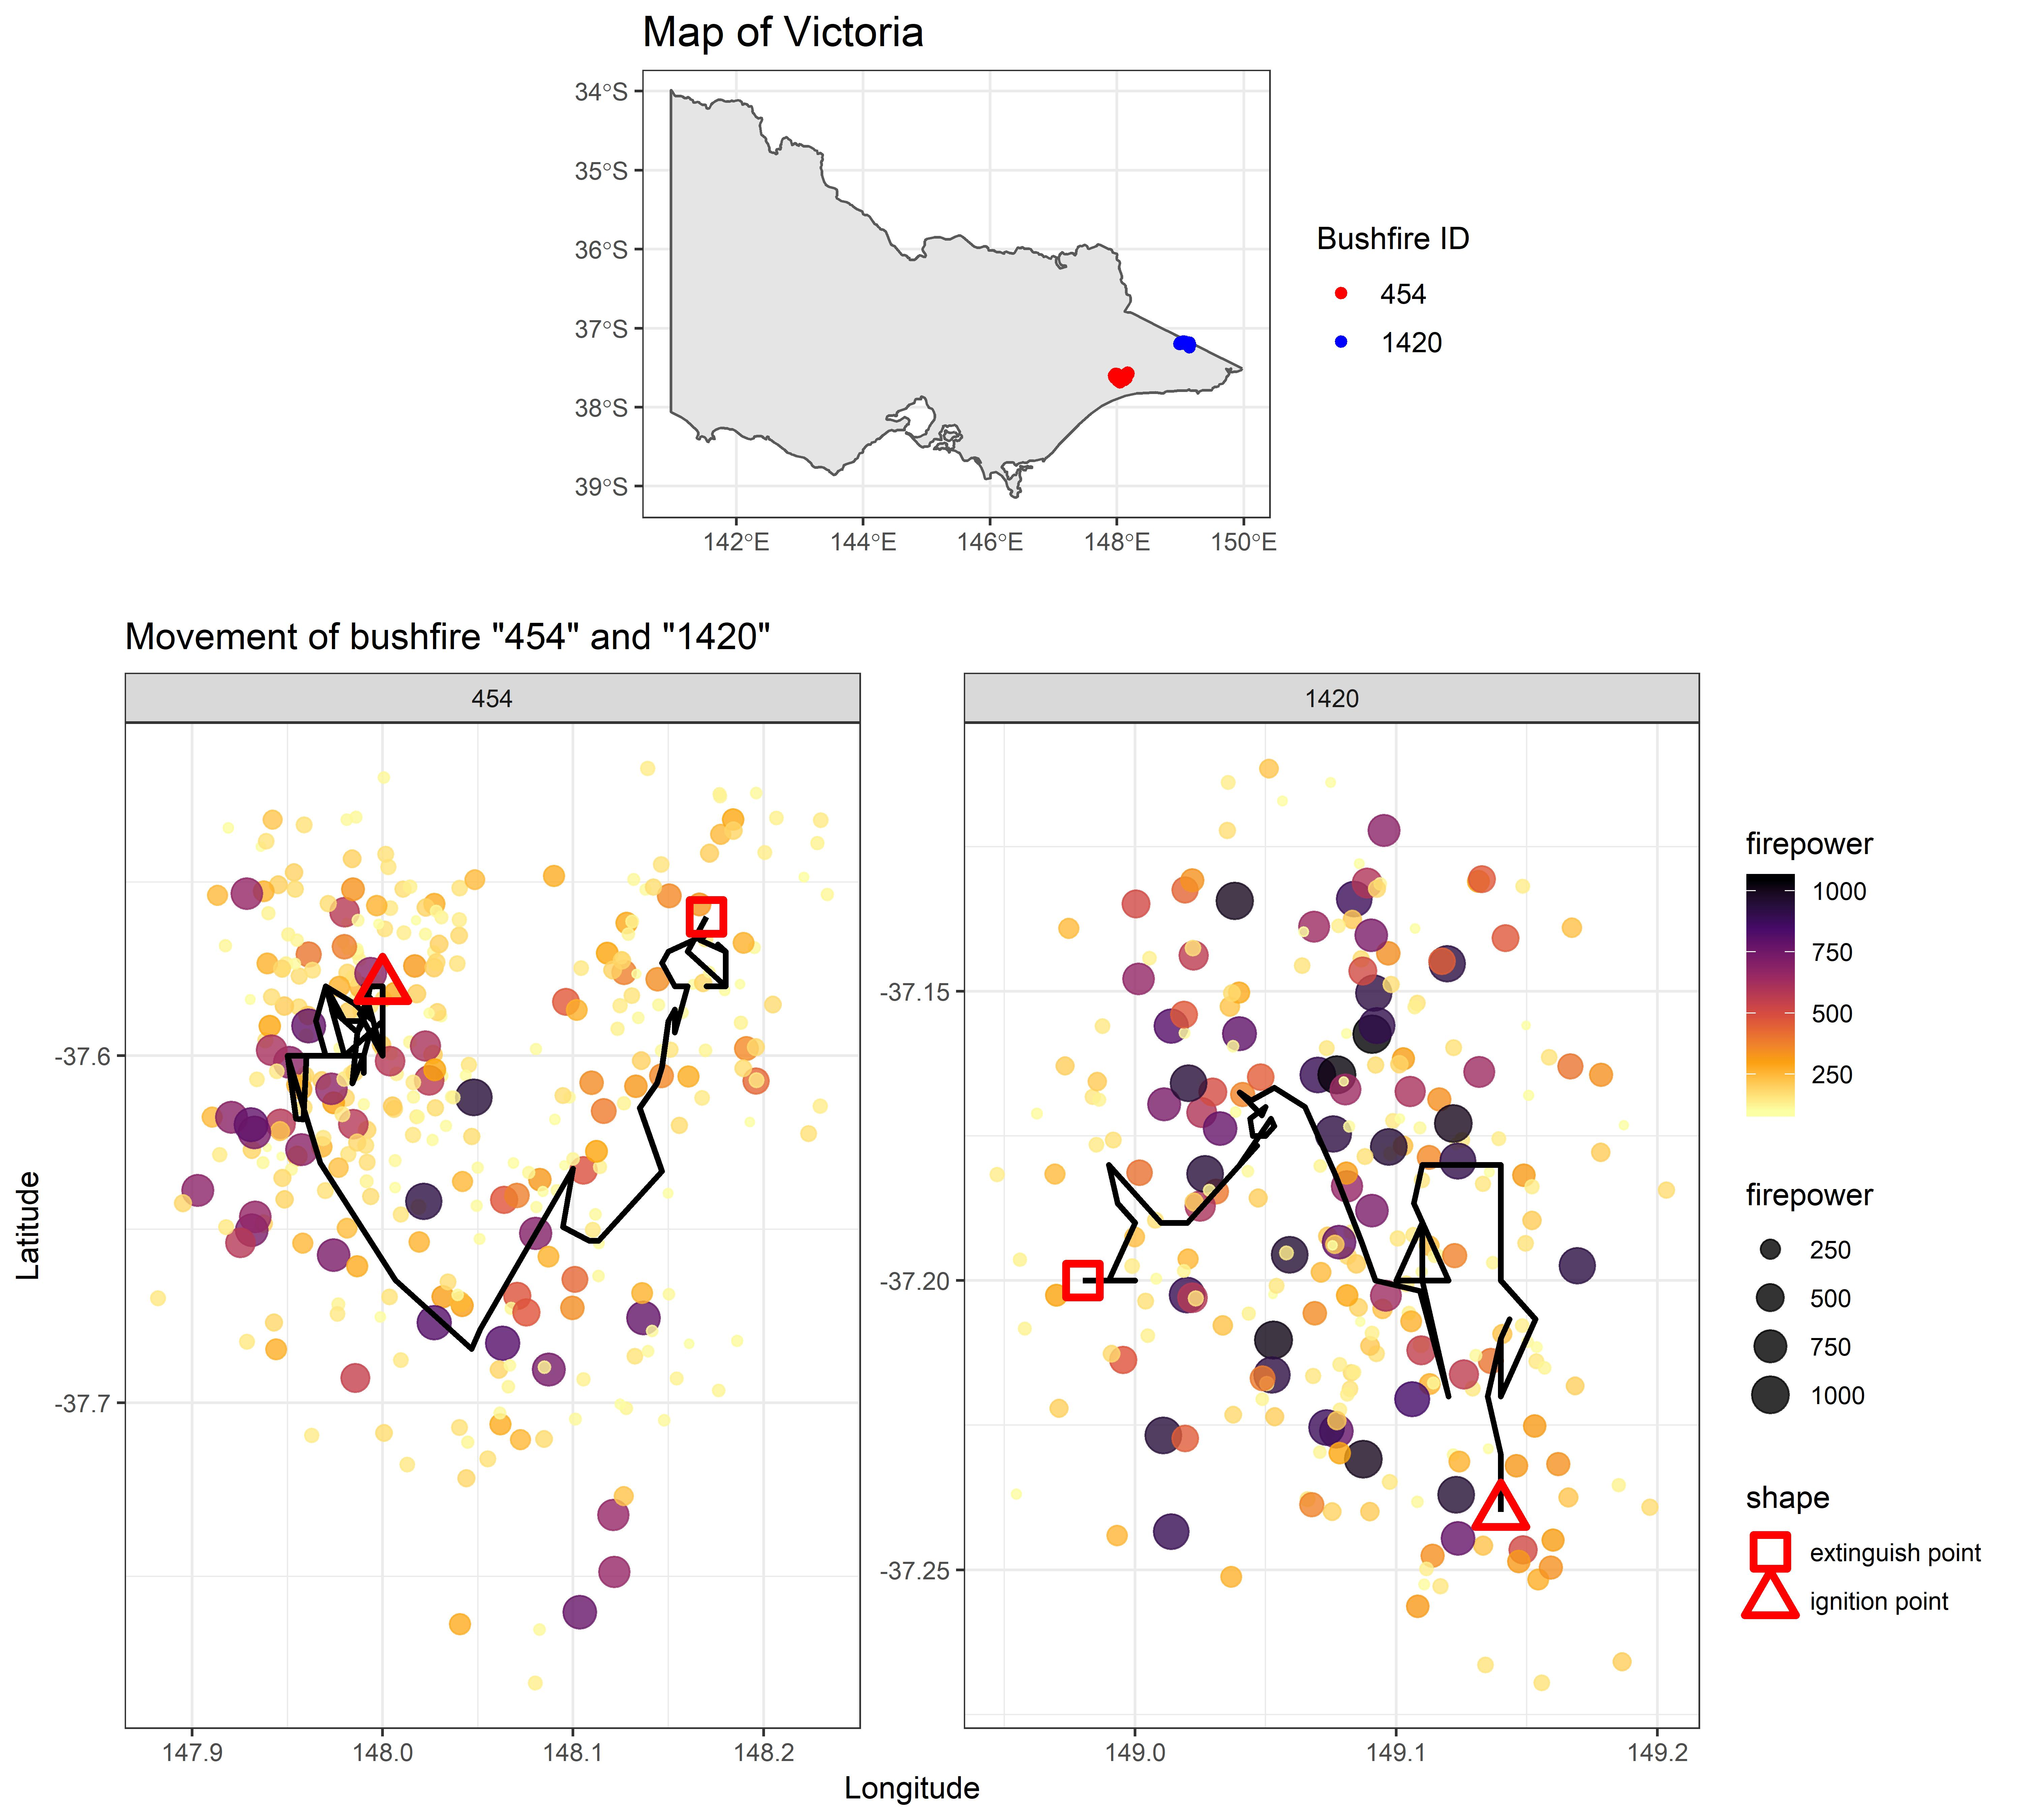
\includegraphics[width=5.20833in,height=\textheight]{figures/fire_mov.jpg}
\caption{The movement path and hotspots map shows the bushfire behaviour of bushfire ``454'' and bushfire ``1420'', which is two clusters from the results of clustering algorithm. The triangle is the ignition point of bushfire and the rectangle is the extinguish point. The black line is the movement of bushfire centeroid. points with red color and larger size are hotspots with higher firepower which is measured by watt per square metre. We can know that bushfires ignited with low firepower, and will getting hotter when time pass, then finally extinguish with not enough fuel. \label{fig:mov}}
\end{figure}

\normalfont
\begin{table}
\caption{\label{tab:clustering}A clustering algorithm for hotspots}
\begin{align*}
&\rule{150mm}{0.5mm}\\[-1\jot]
&\textbf{Algorithm 1 Hotspots clutering}\\[-1\jot]
&\rule{150mm}{0.5mm}\\[-1\jot]
&\textbf{input: }~~~~\text{Hotspots dataset H : (Hour}\textunderscore \text{id}^{(n)} \text{, Coordinates}^{(n)} \text{), n = 1, 2, ... N}\\[-1\jot]
&~~~~~~~~~~~~~~~~\text{An empty dataset F : (Fire\textunderscore id}^{(m)} \text{, Coordinates}^{(m)} \text{, Active}^{(m)} \text{), m = 1, 2, ...}\\[-1\jot]
&~~~~~~~~~~~~~~~~\text{An empty vector K} \in \mathbb{N}_1^n\\[-1\jot]
&~~~~~~~~~~~~~~~~\text{A distance hyperparameter }r_0 \in \mathbb{R}^+\\[-1\jot]
&~~~~~~~~~~~~~~~~\text{A time hyperparameter }t_0 \in \mathbb{N}^+\\[-1\jot]
&\textbf{output: }~~\text{A vector K} \in \mathbb{N}_1^n~\text{contains memberships of hotspots}\\[-1\jot]
&~~~~~~~~~~~~~~~~\text{A dataset F contains fire clusters information including memberships, latest}\\[-1\jot]
&~~~~~~~~~~~~~~~~\text{centroids and time from last updated}\\[-1\jot]
&~~1:~~\text{select subset }H_c \in \text{H where Hour\textunderscore id == 1}\\[-1\jot]
&~~2:~~\text{calculate distance matrix D for Coordinates in }H_c \\[-1\jot]
&~~3:~~\text{assign 1 to a zero adjacency matrix A for where D} \leq r_0~~//~~\text{hotspots with relative}\\[-1\jot]
&~~~~~~~~~\text{distance less or equal to }r_0~\text{will be considered belong to the same cluster} \\[-1\jot]
&~~4:~~\text{create undirected unweighted graph G from A}\\[-1\jot]
&~~5:~~\text{record memberships of G to K}\\[-1\jot]
&~~6:~~\text{record clusters classes to Fire\textunderscore id and record clusters centroids to Coordinates of F}\\[-1\jot]
&~~7:~~\text{set Active in F to }t_0~~//~~\text{Active clusters are fire being observed in the last }t_0~\text{hour}\\[-1\jot]
&~~8:~~\textbf{for}~~\text{hour = 2, ... T}~~\textbf{do} \\[-1\jot]
&~~9:~~~~~~~~\text{let Active -1 and select subset }F_c \in \text{F where Active} \geq 0\\[-1\jot]
&10:~~~~~~~~\text{select subset }H_c \in \text{H where Hour\textunderscore id == hour}\\[-1\jot]
&11:~~~~~~~~\text{append Coordinates from }F_c~\text{to}~H_c\\[-1\jot]
&12:~~~~~~~~\text{repeat step 2 - 4}\\[-1\jot]
&12:~~~~~~~~\textbf{for}~~h_i = \text{each hotspot in }H_c~~\textbf{do}\\[-1\jot]
&13:~~~~~~~~~~~~~~\textbf{if}~~h_i~\text{share the same membership as one of active clusters in }F_c~~\textbf{then}\\[-1\jot]
&14:~~~~~~~~~~~~~~~~~~~~\text{copy the corresponding Fire\textunderscore id of the nearest active cluster to K}\\[-1\jot]
&15:~~~~~~~~~~~~~~\textbf{else}~~\text{copy the membership from G to K}\\[-1\jot]
&16:~~~~~~~~~~~~~~\textbf{end if}\\[-1\jot]
&17:~~~~~~~~\textbf{end for}\\[-1\jot]
&18:~~~~~~~~\text{update F for clusters involved in current time-stamp and reset corresponding}\\[-1\jot]
&~~~~~~~~~~~~~~~\text{Active to }t_0\\[-1\jot]
&19:~~\textbf{end for}\\[-1\jot]
&\rule{150mm}{0.5mm}
\end{align*}
\end{table}

\begin{figure}
\centering
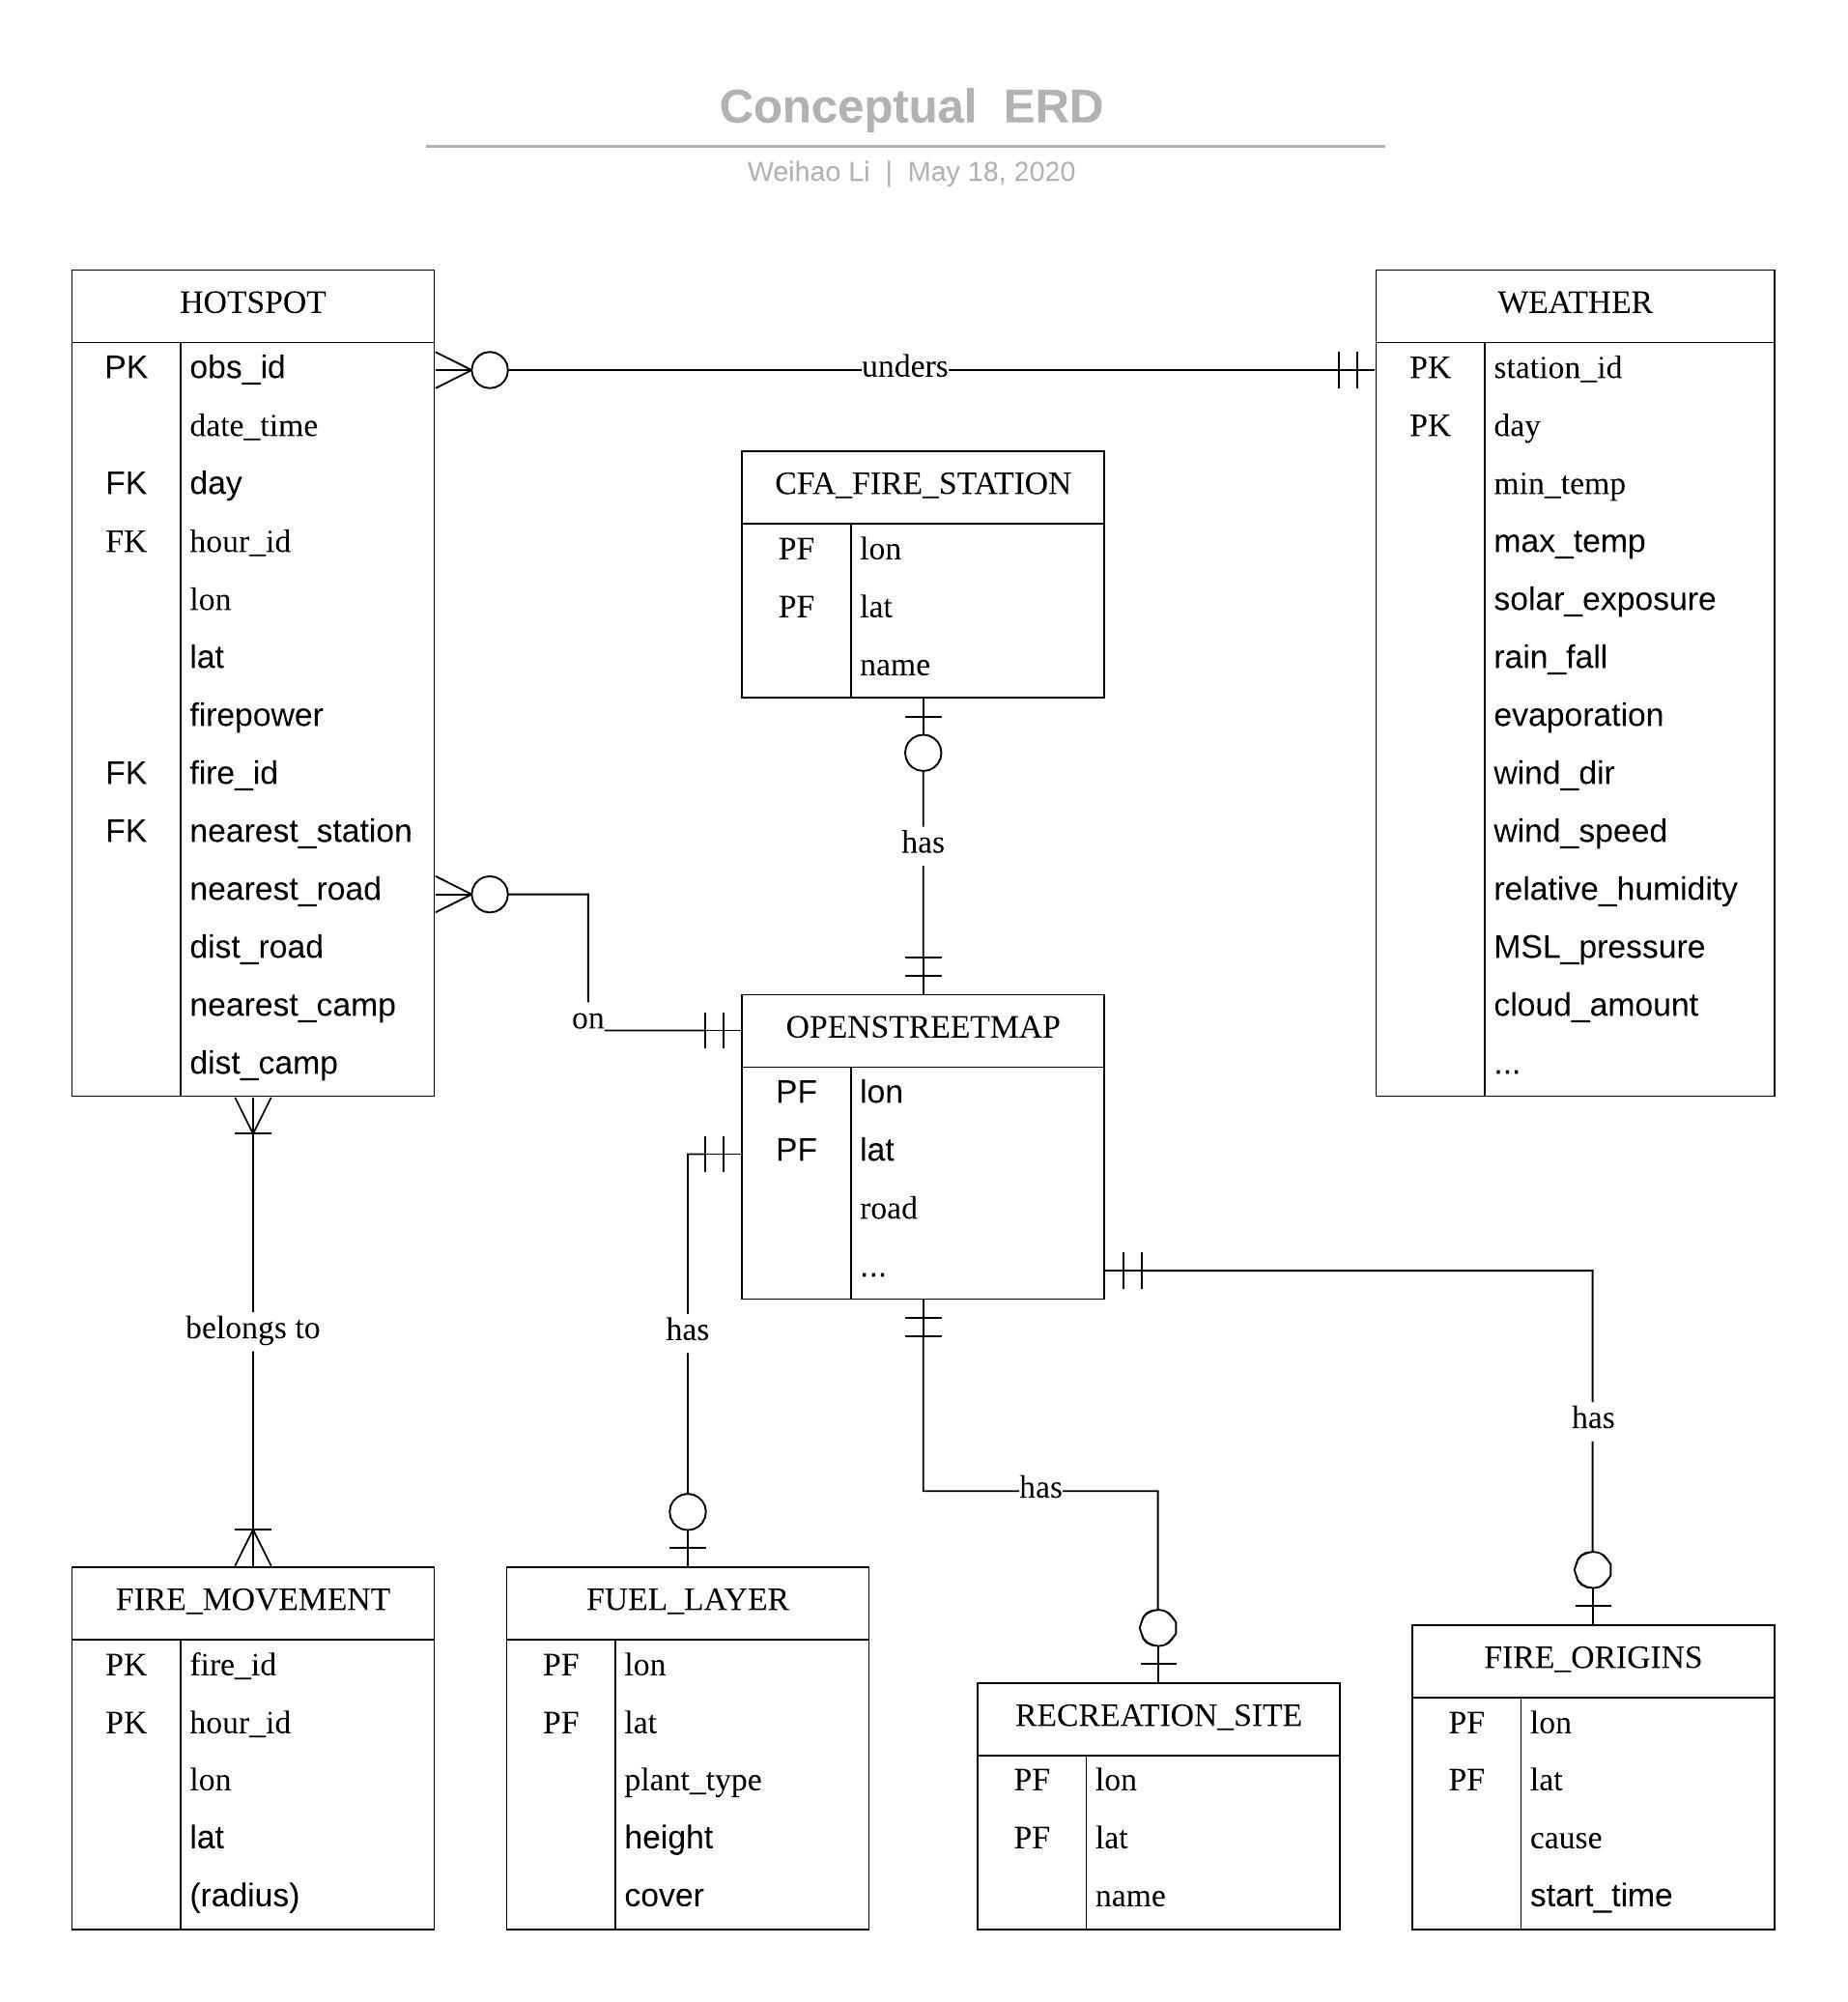
\includegraphics{figures/Shiny_app_data_Conceptual_ERD.jpeg}
\caption{Entity relationship diagram illustrating the relational tables of the compiled data. Tables correspond to processed hotspot data, weather, local facilities like CFA sites. This data structure is useful for the data modeling and web app development. \label{fig:ERD}}
\end{figure}

\begin{figure}
\centering
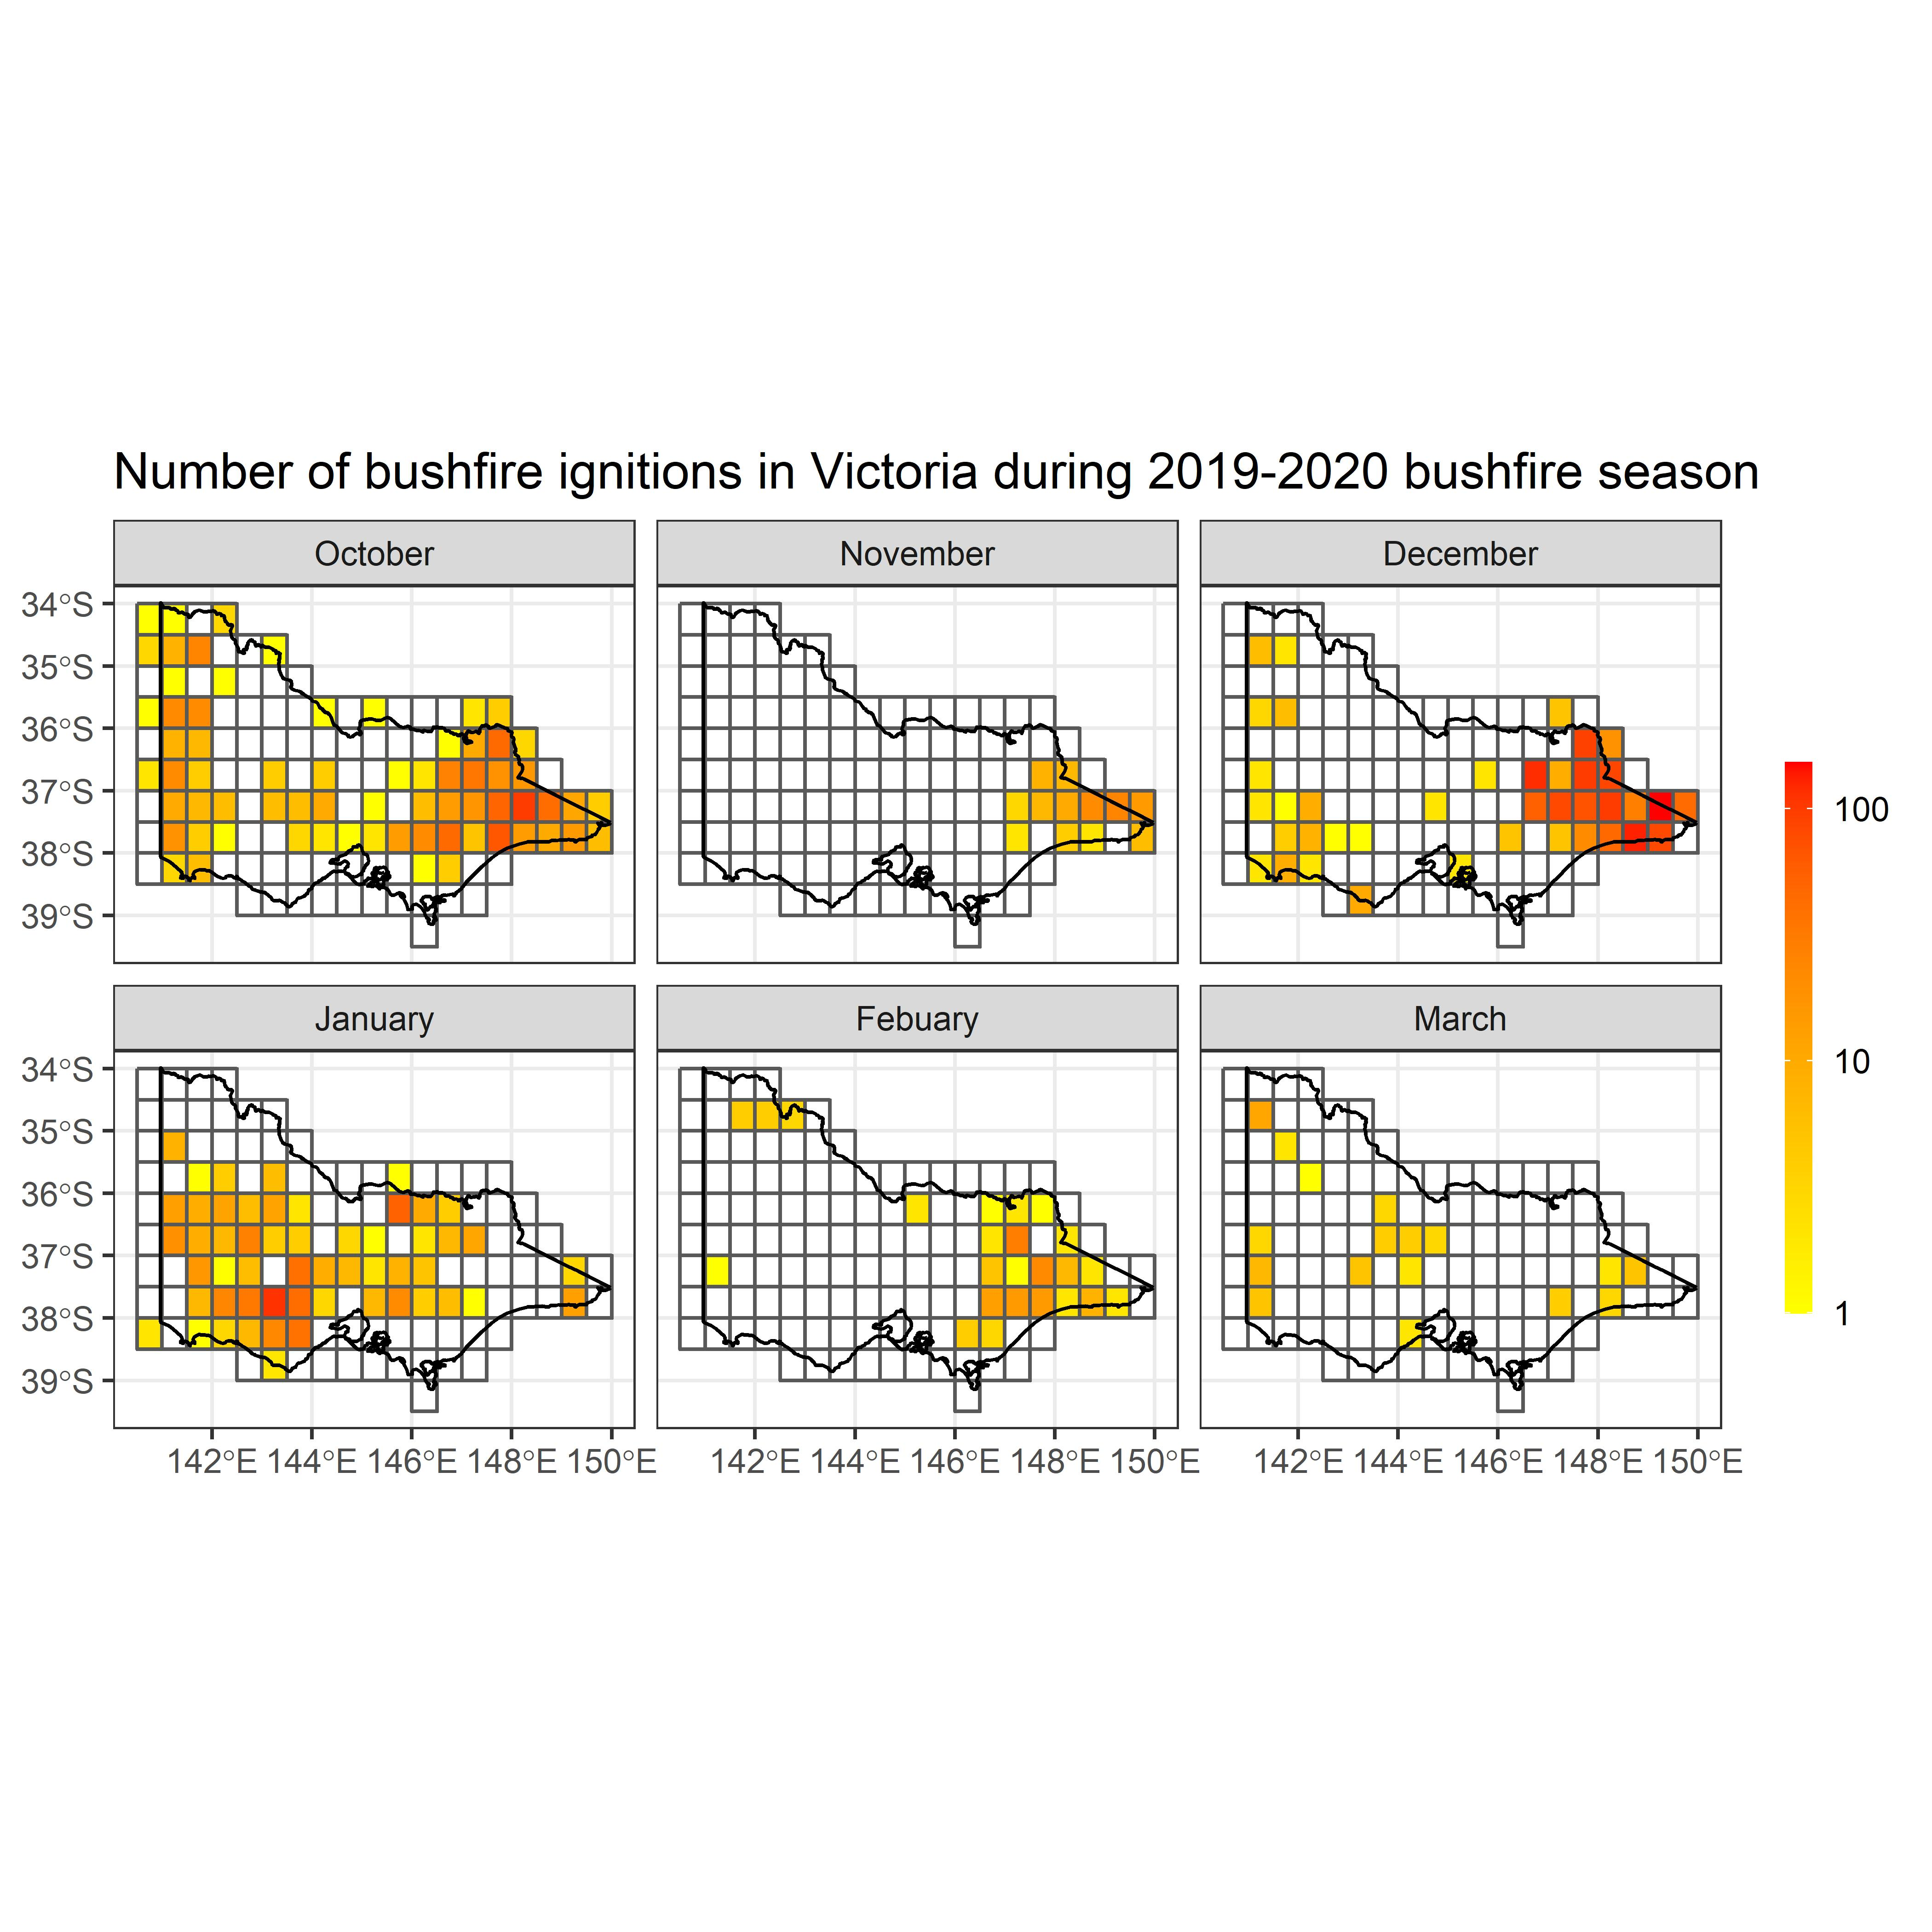
\includegraphics[width=5.20833in,height=\textheight]{figures/number_of_ignitions.jpg}
\caption{The grid map illustrating the general situation of Victoria during 2019-2020 Australia bushfire season. The severest time for Victoria was December when the massive amount of bushfires ignited in Eastern Victoria. Places like East Gippsland suffered from this devastating crisis. \label{fig:overview}}
\end{figure}

\clearpage

\printbibliography

\end{document}

